\documentclass[11pt,a4paper]{article}

% --- Page margins and paragraphs ---
\usepackage[margin=1in]{geometry}
\usepackage{parskip}

% --- Basic math and typesetting ---
\usepackage{amsmath,amssymb,amsthm}
\usepackage{mathtools} % provides \coloneqq
\usepackage{xcolor} % 
\usepackage{graphicx} % for the included figures

% --- Theorem and definition environments ---
\theoremstyle{definition}
\newtheorem{definition}{Definition}
\newtheorem{example}{Example}
\newtheorem{remark}{Remark}

\theoremstyle{plain}
\newtheorem{theorem}{Theorem}
\newtheorem{proposition}{Proposition}
\newtheorem{lemma}{Lemma}


\begin{document}

% ==================================================
% Title and author information
% ==================================================
\begin{center}
    {\LARGE \textbf{Mathematics Method for Physics--Lecture 2}} \\[0.6em]
    {\large Point Sets in the Complex Plane}
\end{center}

\vspace{-0.5em}
\noindent\rule{\textwidth}{0.5pt}
\vspace{0.3em}

\begin{center}
    Instructor: Zhaolong Han, SOCE, Shanghai Jiao Tong University;
\end{center}

\vspace{-0.6em}
\noindent Email: han.arkey@sjtu.edu.cn

\vspace{0.4em}
\noindent\rule{\textwidth}{0.5pt}

\vspace{0.8em}
% Blue hint/explanation text
\noindent { Start up saying}

\vspace{1.5em}

% ==================================================
% Main content
% ==================================================
Lecture 1 treated a complex number as a single object. The present chapter instead studies \textbf{subsets} of $\mathbb{C}$, that is, collections of points of the plane rather than individual points. The properties examined below all refer to the position of the points of such a set, not to the algebra of the complex numbers themselves, and they are what will later allow a function to be studied on a region rather than at a single point.

\section{Neighborhoods}

The basic measuring tool is the open disk.

\begin{definition}[$\delta$-neighborhood]
The $\delta$\textbf{-neighborhood} of a point $z_0 \in \mathbb{C}$ is the open disk
\begin{equation}
U(z_0, \delta) \coloneqq \{ z \in \mathbb{C} : |z - z_0| < \delta \}, \quad \delta > 0.
\end{equation}
Its boundary circle $|z - z_0| = \delta$ is \textbf{not} part of $U(z_0, \delta)$. Removing the centre as well gives the \textbf{punctured (deleted) neighborhood}
\begin{equation}
\mathring{U}(z_0, \delta) \coloneqq \{ z \in \mathbb{C} : 0 < |z - z_0| < \delta \},
\end{equation}
which is the natural setting for limits, where the value at $z_0$ itself must not influence the behaviour.
\end{definition}

Every definition in this chapter has one of two logical forms: it requires a property to hold \textit{for all sufficiently small $\delta > 0$}, or it requires the existence of \textit{at least one $\delta > 0$} with that property. Distinguishing the two forms is the main point of the definitions that follow.

\section{Interior, Exterior and Boundary Points}

\begin{remark}[Complement]
The \textbf{complement} of $E$ in $\mathbb{C}$ is the set of points of the plane that do not belong to $E$:
\begin{equation}
\mathbb{C} \setminus E \coloneqq \{ z \in \mathbb{C} : z \notin E \}.
\end{equation}
The complement is defined relative to the ambient set $\mathbb{C}$, so $E \cup (\mathbb{C} \setminus E) = \mathbb{C}$ and $E \cap (\mathbb{C} \setminus E) = \varnothing$. The notation below uses it only in this sense.
\end{remark}

Let $E \subset \mathbb{C}$ be a point set and $z_0 \in \mathbb{C}$. Relative to $E$, the point $z_0$ is exactly one of the following.
\begin{enumerate}
    \item \textbf{Interior point:} $z_0 \in E$ and there is a $\delta > 0$ such that
    \begin{equation}
    U(z_0, \delta) \subset E.
    \end{equation}
    \item \textbf{Exterior point:} there is a $\delta > 0$ such that
    \begin{equation}
    U(z_0, \delta) \cap E = \varnothing.
    \end{equation}
    \item \textbf{Boundary point:} for \textbf{every} $\delta > 0$,
    \begin{equation}
    U(z_0, \delta) \cap E \ne \varnothing \quad \text{and} \quad U(z_0, \delta) \cap (\mathbb{C} \setminus E) \ne \varnothing.
    \end{equation}
\end{enumerate}

\begin{figure}[htbp]
    \centering
    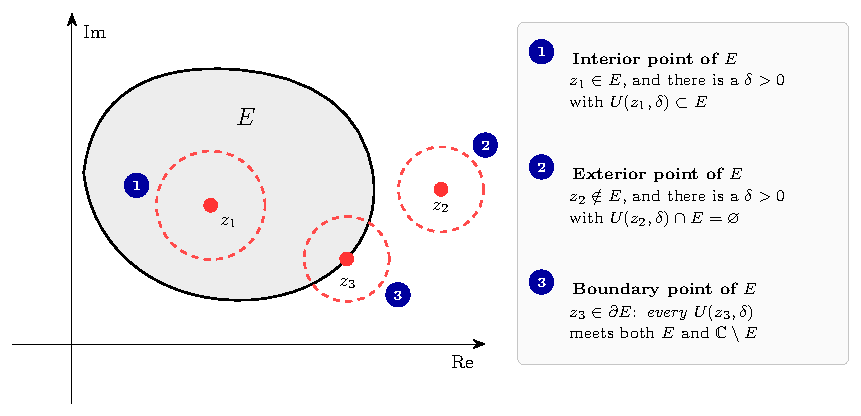
\includegraphics[width=\textwidth]{figs/fig01-interior-exterior-boundary.pdf}
    \caption{Interior point $z_1$, exterior point $z_2$ and boundary point $z_3$ of a set $E$. The dashed circle is the $\delta$-neighborhood of the marked point.}
    \label{fig:interior-exterior-boundary}
\end{figure}

As Figure~\ref{fig:interior-exterior-boundary} shows, the interior point $z_1$ has a whole disk that stays inside $E$; the exterior point $z_2$ has a whole disk that avoids $E$; the boundary point $z_3$ has no such disk, since every disk around it is split between $E$ and its complement. Note:
\begin{itemize}
    \item The three cases are \textbf{mutually exclusive and exhaustive}: every point of $\mathbb{C}$ is interior, exterior, or boundary.
    \item An interior point necessarily lies in $E$, and an exterior point necessarily lies outside $E$; a boundary point may lie either in $E$ or outside it. The boundary is therefore \textit{not} required to belong to $E$ or to $\mathbb{C} \setminus E$.
    \item An \textbf{isolated point} of $E$ (a point of $E$ with some $\mathring{U}(z_0, \delta) \cap E = \varnothing$) is always a boundary point, because $U(z_0, \delta)$ still meets $E$ at $z_0$ itself.
\end{itemize}

\section{Boundary, Interior, Open and Closed Sets}

Collecting the three kinds of points gives three sets:
\begin{equation}
E^{\circ} \coloneqq \{ z : z \text{ is an interior point of } E \},
\end{equation}
\begin{equation}
\partial E \coloneqq \{ z : z \text{ is a boundary point of } E \},
\end{equation}
\begin{equation}
\operatorname{ext} E \coloneqq \{ z : z \text{ is an exterior point of } E \}.
\end{equation}
$E^{\circ}$ is the \textbf{interior} of $E$ and $\partial E$ is the \textbf{boundary} of $E$. By the last relation, the exterior is just the interior of the complement, $\operatorname{ext} E = (\mathbb{C} \setminus E)^{\circ}$. Adding the boundary to $E$ produces the \textbf{closure}
\begin{equation}
\overline{E} \coloneqq E \cup \partial E,
\end{equation}
which is the smallest set that contains $E$ and all of its boundary points. It is called the closure because of the next property: a set is closed exactly when it already contains its boundary, and then $\overline{E} = E$.

\begin{figure}[htbp]
    \centering
    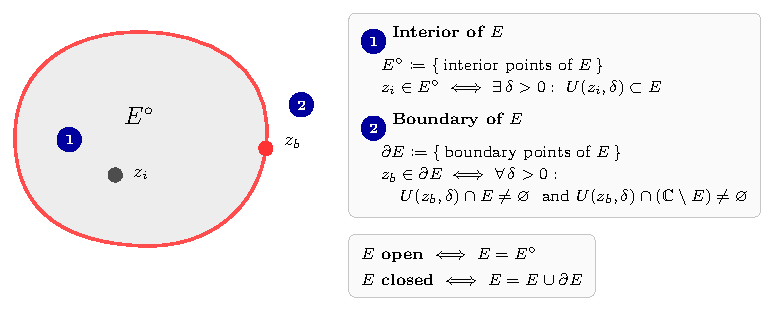
\includegraphics[width=\textwidth]{figs/fig02-boundary-open-closed.pdf}
    \caption{The boundary $\partial E$ (red) and the interior $E^{\circ}$ of a set $E$, together with the definitions of an open and of a closed set.}
    \label{fig:boundary-open-closed}
\end{figure}

A set is classified by how much of its own boundary it carries (Figure~\ref{fig:boundary-open-closed}).
\begin{itemize}
    \item $E$ is \textbf{open} if and only if every one of its points is interior, i.e.
    \begin{equation}
    E \ \text{open} \iff E = E^{\circ}.
    \end{equation}
    \item $E$ is \textbf{closed} if and only if it contains its whole boundary, i.e.
    \begin{equation}
    E \ \text{closed} \iff E = \overline{E} = E \cup \partial E.
    \end{equation}
    \item Equivalently, $E$ is closed exactly when its complement is open:
    \begin{equation}
    E \ \text{closed} \iff \mathbb{C} \setminus E \ \text{open}.
    \end{equation}
\end{itemize}

The two notions are not opposites. Take $E = \{ z : |z| < 1 \} \cup \{ 1 \}$: the point $1$ lies in $E$ but has no neighborhood inside $E$, so $E$ is not open, while $\partial E = \{ z : |z| = 1 \}$ is not contained in $E$, so $E$ is not closed either. ``Open'' forbids boundary points, ``closed'' demands all of them, and a set may fail both tests at once. Note that a circle $\{ z : |z| = 1 \}$, taken as a set of points, \textit{is} closed --- it equals its own boundary --- although it has empty interior.

Consequently, $E$ is open if and only if $\partial E \cap E = \varnothing$, and $E$ is closed if and only if $\partial E \subset E$. Moreover $\partial E = \partial(\mathbb{C} \setminus E)$, so a set and its complement have the same boundary.

\section{Connected Sets}

A set either is of one piece or falls apart into several. \textbf{Connectedness} is the formal expression of the first alternative: any two of its points can be joined without leaving the set.

\begin{definition}[Polygonal path, connected set]
A \textbf{polygonal path} in $E$ joining $z_1$ and $z_2$ is a union of finitely many segments whose vertices start at $z_1$ and end at $z_2$:
\begin{equation}
\gamma = \bigcup_{k=1}^{n} [w_{k-1}, w_k], \qquad w_0 = z_1, \quad w_n = z_2, \quad [w_{k-1}, w_k] \subset E.
\end{equation}
$E$ is \textbf{connected} if every two of its points can be so joined:
\begin{equation}
E \ \text{connected} \iff \forall\, z_1, z_2 \in E \ \ \exists\, \gamma \subset E \ \text{joining} \ z_1 \ \text{to} \ z_2.
\end{equation}
\end{definition}

\begin{figure}[htbp]
    \centering
    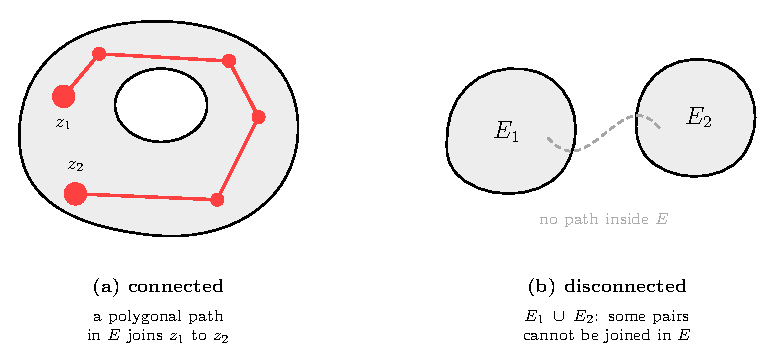
\includegraphics[width=\textwidth]{figs/fig03-connected-disconnected.pdf}
    \caption{(a) A region with a hole is still connected: the polygonal path joins $z_1$ to $z_2$ while going around the hole. (b) $E_1 \cup E_2$ is disconnected, since no path inside the set bridges the gap.}
    \label{fig:connected-disconnected}
\end{figure}

In Figure~\ref{fig:connected-disconnected}(a) the region is not simply shaped, yet it remains \textbf{connected}, since the polygonal path joining $z_1$ to $z_2$ avoids the hole. A hole therefore does not destroy connectedness; only a genuine separation does, as in Figure~\ref{fig:connected-disconnected}(b), where $E_1 \cup E_2$ falls into two components and no path inside the set joins them.

\section{Domains and Connectivity}

Combining the last two sections gives the central object of the whole course.

\begin{definition}[Domain, region, closed domain]
A \textbf{domain} (or \textbf{region}) $D$ is a point set that is both open and connected:
\begin{equation}
D \ \text{domain} \iff D \ \text{open and connected}.
\end{equation}
A domain is \textbf{bounded} if $D \subset U(0, R)$ for some $R > 0$, and \textbf{unbounded} otherwise. A domain together with its boundary, $\overline{D} = D \cup \partial D$, is called a \textbf{closed domain}.
\end{definition}

Openness is what distinguishes a domain from an arbitrary set: it is the property that lets a neighbourhood be placed around every one of its points, and it is exactly what will later be needed to speak about a limit taken at a point of the set. Connectedness is the separate requirement that the set not fall into unrelated components. Every domain is an open set, but the converse fails: for $z_0 \ne z_1$ the set $U(z_0, \delta) \cup U(z_1, \delta)$ is open and yet is not a domain, being disconnected. Openness is a \textit{local} property, verified one neighborhood at a time; being a domain also requires the \textit{global} property that the set be of one piece.

Domains are further distinguished by the number of holes they enclose. $D$ is \textbf{simply connected} if every closed curve lying in $D$ can be shrunk continuously to a single point without ever leaving $D$:
\begin{equation}
C \subset D, \ C \ \text{a closed curve} \ \Longrightarrow \ C \ \text{contracts to a point inside} \ D.
\end{equation}
Otherwise $D$ is \textbf{multiply connected}.

\begin{figure}[htbp]
    \centering
    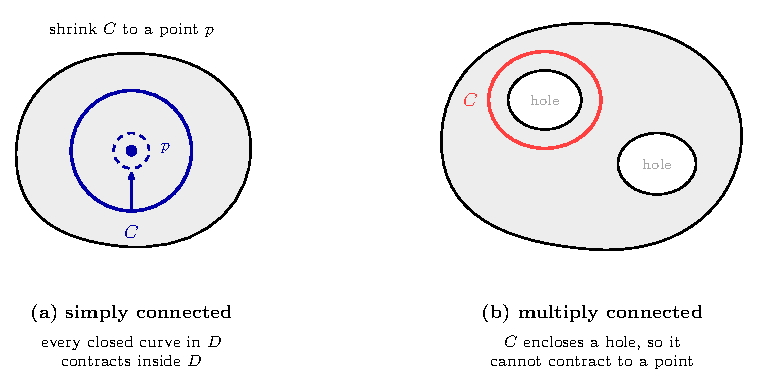
\includegraphics[width=\textwidth]{figs/fig04-simply-multiply-connected.pdf}
    \caption{(a) In a simply connected domain every closed curve $C$ contracts within $D$ to a point $p \in D$. (b) In a multiply connected domain a closed curve $C$ may enclose a hole, and then it cannot be contracted within $D$.}
    \label{fig:simply-multiply-connected}
\end{figure}

In Figure~\ref{fig:simply-multiply-connected}(a) the curve $C$ contracts within $D$ to a point $p \in D$. In Figure~\ref{fig:simply-multiply-connected}(b) the curve $C$ encircles a hole; contracting it to a point would require it to cross that hole, which does not belong to $D$. A simply connected domain is thus one without holes, equivalently one whose complement $\mathbb{C} \setminus D$ has no bounded component.

The two notions must be kept apart. An annulus is connected, since any two of its points can be joined by a path inside it, yet it is multiply connected. Connectedness concerns the existence of paths between points; simple connectedness concerns the contractibility of closed curves.

\section{Positive Orientation of the Boundary}

For a domain with holes, or an unbounded domain, the boundary $\partial D$ may consist of several separate closed curves. To treat $\partial D$ as a single object, these curves have to be traversed in a coherent order.

\begin{definition}[Positively oriented boundary]
The \textbf{positively oriented boundary} $\Gamma^{+}$ of a domain $D$ is the traversal of $\partial D$ for which the domain stays on the \textbf{left}:
\begin{equation}
\Gamma^{+} : \quad D \ \text{lies to the left of the direction of travel}.
\end{equation}
The opposite traversal is written $\Gamma^{-}$.
\end{definition}

For a disk domain there is a single boundary curve, and the rule forces it to be counterclockwise (Figure~\ref{fig:positive-boundary}):
\begin{equation}
\Gamma = C_0 \quad (\text{counterclockwise}).
\end{equation}
For a circular-ring domain the boundary has two components, and the rule forces opposite senses: the outer circle counterclockwise, the inner circle clockwise,
\begin{equation}
\Gamma = C_0 + C_1^{-} \quad (\text{outer ccw}, \ \text{inner cw}).
\end{equation}

\begin{figure}[htbp]
    \centering
    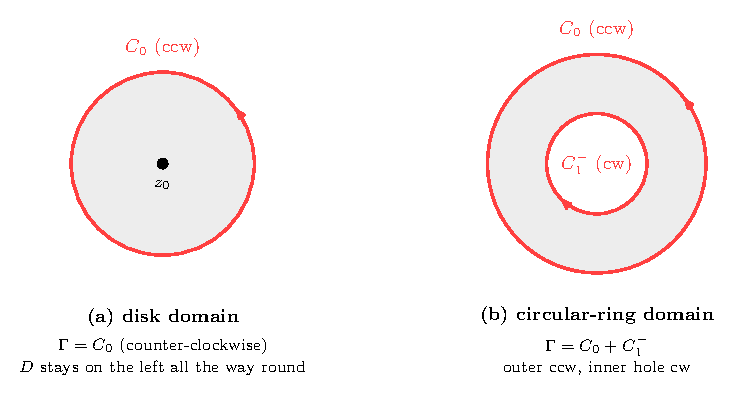
\includegraphics[width=\textwidth]{figs/fig05-positive-boundary.pdf}
    \caption{Positive orientation. (a) For a disk domain the boundary $C_0$ is traversed counterclockwise. (b) For a circular-ring domain the outer circle $C_0$ is traversed counterclockwise and the inner hole $C_1^{-}$ clockwise, so that $D$ stays on the left throughout.}
    \label{fig:positive-boundary}
\end{figure}

Here the superscript minus in $C_1^{-}$ denotes traversal in the reversed, clockwise sense. This is the unique choice for which $D$ lies to the left along \textbf{every} component, so that the several curves combine into a single positively oriented boundary instead of partly cancelling each other.

The same rule extends to a domain with $n$ holes, giving one outer curve and $n$ inner curves (Figure~\ref{fig:n-hole-boundary}):
\begin{equation}
\Gamma = C_0 + C_1^{-} + C_2^{-} + \cdots + C_n^{-}.
\end{equation}

\begin{figure}[htbp]
    \centering
    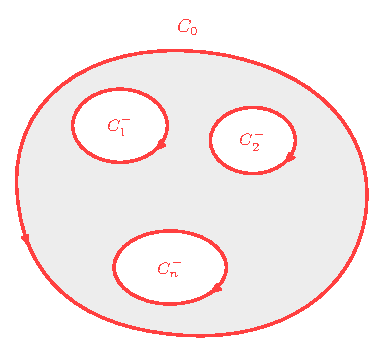
\includegraphics[width=0.72\textwidth]{figs/fig06-n-hole-boundary.pdf}
    \caption{The boundary of a domain with $n$ holes. The outer boundary $C_0$ is traversed counterclockwise and every hole $C_1^{-}, \dots, C_n^{-}$ clockwise, so that the domain always stays on the left.}
    \label{fig:n-hole-boundary}
\end{figure}

\section{The Extended Complex Plane}

The complex plane is not large enough to give every sequence a limit: the sequence $z_k = k$ has no limit in $\mathbb{C}$, since its terms leave every disk $U(0, R)$. Adjoining a single ideal point repairs this.

\begin{definition}[Extended complex plane]
The \textbf{extended complex plane} is
\begin{equation}
\widehat{\mathbb{C}} \coloneqq \mathbb{C} \cup \{ \infty \}.
\end{equation}
\end{definition}

We write $|\infty| = +\infty$, but no arithmetic is defined for $\infty$: expressions such as $\infty - \infty$ or $0 \cdot \infty$ remain meaningless. The point $\infty$ is a \textit{location}, not a number.

A set of the form
\begin{equation}
\{ z \in \mathbb{C} : |z| > R \} \cup \{ \infty \}, \quad R > 0,
\end{equation}
is a \textbf{neighborhood of $\infty$}. With this definition $\infty$ behaves like any other point of $\widehat{\mathbb{C}}$: it has neighborhoods, and a sequence diverges to $\infty$ exactly when it eventually lies in every such neighborhood. A set $E \subset \mathbb{C}$ is bounded precisely when its closure in $\widehat{\mathbb{C}}$ does not contain $\infty$.

The geometric model of $\widehat{\mathbb{C}}$ is the \textbf{Riemann sphere}. Take the unit sphere
\begin{equation}
\Sigma : \ X^2 + Y^2 + Z^2 = 1
\end{equation}
and identify the plane $\mathbb{C}$ with the equatorial plane $Z = 0$. \textbf{Stereographic projection} sends $z = x + \mathrm{i} y$ to the point where the line from the north pole $N = (0,0,1)$ through $(x,y,0)$ meets $\Sigma$:
\begin{equation}
X = \frac{2x}{1 + |z|^2}, \quad
Y = \frac{2y}{1 + |z|^2}, \quad
Z = \frac{|z|^2 - 1}{1 + |z|^2}.
\end{equation}
The map is a bijection from $\mathbb{C}$ onto $\Sigma \setminus \{ N \}$. The inverse is
\begin{equation}
x = \frac{X}{1 - Z}, \quad y = \frac{Y}{1 - Z},
\end{equation}
and completing it by $N \mapsto \infty$ extends the correspondence to all of $\widehat{\mathbb{C}}$:
\begin{equation}
\widehat{\mathbb{C}} \ \longleftrightarrow \ \Sigma, \qquad \infty \ \longleftrightarrow \ N.
\end{equation}

\begin{figure}[htbp]
    \centering
    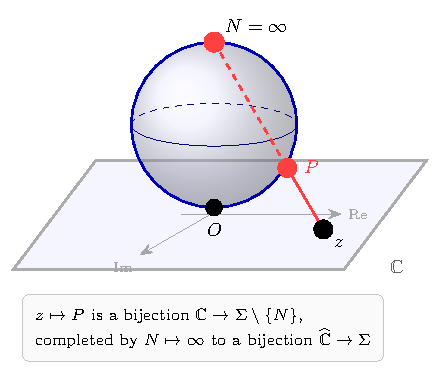
\includegraphics[width=0.58\textwidth]{figs/fig07-riemann-sphere.pdf}
    \caption{Stereographic projection. The line from the north pole $N$ through a point $z$ of the plane meets the sphere at $P$, and $N$ itself corresponds to $\infty$. The dashed half of the equator is the part of the sphere behind the plane.}
    \label{fig:riemann-sphere}
\end{figure}

Since the map is continuous in both directions, $\widehat{\mathbb{C}}$ may be read as $\Sigma$ and questions about $\infty$ become questions about the north pole. This is what makes it possible to treat $\infty$ as an ordinary point of the plane's compactification rather than as a separate exception.

Two consequences are used later. First, a circle $|z| = R$ in the plane corresponds to a circle of latitude on the sphere,
\begin{equation}
|z|^2 = \frac{1 + Z}{1 - Z} \quad \Longleftrightarrow \quad Z = \frac{R^2 - 1}{R^2 + 1},
\end{equation}
so that $R \uparrow \infty$ drives $Z \uparrow 1$: the exterior of a large circle is exactly a small neighborhood of the north pole. Second, lines in the plane correspond to circles on $\Sigma$ passing through $N$, so on the sphere ``circle'' and ``line'' merge into a single notion --- the generalized circle.

\section{Worked Examples}

Two loci are examined below. In each case the defining condition is reduced to a system of inequalities between moduli, from which the boundary and the connectivity of the set can be read off.

\subsection{A Lune Bounded by Two Tangent Circles}

\begin{example}[Lune between two tangent circles]
Determine the set
\begin{equation}
D \coloneqq \{ z = r\mathrm{e}^{\mathrm{i}\theta} : \cos\theta < r < 2\cos\theta \}
\end{equation}
and describe its boundary and connectivity.
\end{example}

\noindent\textit{Solution.} The constraint $\cos\theta > r \ge 0$ forces $\cos\theta > 0$, so $\theta \in (-\frac{\pi}{2}, \frac{\pi}{2})$. Multiplying the polar equations by $r > 0$ and using $r^2 = x^2 + y^2$ and $r\cos\theta = x$, the outer curve becomes
\begin{equation}
r = 2\cos\theta \iff r^2 = 2r\cos\theta \iff x^2 + y^2 = 2x \iff |z - 1| = 1,
\end{equation}
and the inner curve becomes
\begin{equation}
r = \cos\theta \iff r^2 = r\cos\theta \iff x^2 + y^2 = x \iff \left|z - \tfrac{1}{2}\right| = \tfrac{1}{2}.
\end{equation}
These are the circles of diameter $[0,2]$ and $[0,1]$, both passing through the origin, where they are internally tangent. Hence
\begin{equation}
D = \{ z : |z - 1| < 1 \} \cap \left\{ z : \left|z - \tfrac{1}{2}\right| > \tfrac{1}{2} \right\},
\end{equation}
the open lune between the two circles.

\noindent\textit{Conclusion.} $D$ is a \textbf{domain}: it is open, both inequalities being strict, and connected. It is \textbf{bounded}, since $D \subset U(0,2)$. It is \textbf{simply connected}: the excluded disk $|z - \frac{1}{2}| \le \frac{1}{2}$ touches the outer circle at the single point $0$, hence it is attached to the exterior of $D$ rather than enclosed by it; the complement of $D$ is therefore connected and $D$ has no hole. The boundary $\partial D = \Gamma_1 \cup \Gamma_2$ is the union of the two circles $\Gamma_1 : |z - \frac{1}{2}| = \frac{1}{2}$ and $\Gamma_2 : |z - 1| = 1$.

\subsection{An Angular Locus}

\begin{example}[An angular locus]
Determine the set
\begin{equation}
D \coloneqq \left\{ z : 0 < \arg\frac{z - \mathrm{i}}{z + \mathrm{i}} < \frac{\pi}{4} \right\}
\end{equation}
and describe its boundary and connectivity.
\end{example}

\noindent\textit{Solution.} Let $\alpha \in (0, \frac{\pi}{2})$ and consider the locus $\arg\frac{z - \mathrm{i}}{z + \mathrm{i}} = \alpha$. It consists of the points from which the segment joining $-\mathrm{i}$ to $+\mathrm{i}$ subtends the angle $\alpha$. By the inscribed-angle theorem, the same circle geometry that underlies Thales's theorem in Lecture 1, a fixed chord is seen under a fixed angle exactly on an \textbf{arc of a circle} through its endpoints, and that circle is determined by the condition that the central angle equal $2\alpha$.

For $\alpha = \frac{\pi}{4}$ the chord $[-\mathrm{i}, \mathrm{i}]$ has length $2$, so the circle has radius $R$ with $2R\sin\frac{\pi}{4} = 2$, giving $R = \sqrt{2}$. Its centre lies on the real axis, and passing through $\pm\mathrm{i}$ forces the centre to be $-1$:
\begin{equation}
|z + 1| = \sqrt{2}.
\end{equation}
This circle passes through $\pm\mathrm{i}$ (since $|\pm\mathrm{i} + 1| = \sqrt{2}$) and meets the real axis at $-1 \pm \sqrt{2}$. The limiting case $\alpha = 0$ degenerates to the chord's own line, namely the imaginary axis, minus the segment between the endpoints.

Collecting both pieces, the lower bound $\alpha > 0$ keeps $z$ on the side of the imaginary axis where the angle is measured positively, and the upper bound $\alpha < \frac{\pi}{4}$ keeps $z$ outside the disk:
\begin{equation}
D = \{ z : \operatorname{Re} z < 0 \} \cap \{ |z + 1| > \sqrt{2} \}.
\end{equation}

\noindent\textit{Conclusion.} $D$ is a \textbf{domain}: it is open, both inequalities being strict, and connected --- the disk $|z + 1| \le \sqrt{2}$ cuts a cap out of the left half-plane, but that cap is attached to the boundary line, so $D$ remains of one piece. It is \textbf{unbounded}, since it contains every $z = -R$ with $R > 1 + \sqrt{2}$. It is \textbf{simply connected}: the removed cap touches $\partial D$ along the imaginary axis, so again no hole is enclosed.

The boundary $\partial D = \Gamma_1 \cup \Gamma_2$ consists of the two rays of the imaginary axis outside the chord,
\begin{equation}
\Gamma_1 : \ \operatorname{Re} z = 0, \ |\operatorname{Im} z| \ge 1,
\end{equation}
together with the major arc of the circle $|z + 1| = \sqrt{2}$ that lies in the closed left half-plane,
\begin{equation}
\Gamma_2 : \ |z + 1| = \sqrt{2}, \ \operatorname{Re} z \le 0,
\end{equation}
and the positively oriented boundary traverses both rays of $\Gamma_1$ \textbf{upwards}, then runs along $\Gamma_2$ from $-\mathrm{i}$ around $-1 - \sqrt{2}$ to $+\mathrm{i}$, keeping $D$ on the left throughout. Traversed the other way round, $D$ would fall on the right, so the orientation is forced.

\end{document}